\documentclass[12pt]{article}
\usepackage{mildert-common}
\usepackage{enumerate}
% For making the timeline:
\usepackage{pgffor}
\usepackage{tikz}
\usetikzlibrary{decorations.pathreplacing,positioning}
\usepackage{adjustbox}

\title{Appendix C: Election Candidate Guidance}
\author{Van~Mildert~College Junior~Common~Room}
\newcommand{\thedate}{6th October 2023}
\date{\thedate}

\begin{document}
    \begin{titlepage}  % Title page
        \maketitle
        \begin{figure}[h]
            
\includegraphics[scale=0.25]{arms}  % Coat of arms
            \centering
        \end{figure}
        \thispagestyle{empty}
    \end{titlepage}
    \setcounter{page}{2}  % Correct page numbering

    The Standing Orders provide the authoritative election procedure; Appendix C is supplementary to the Standing Orders.

    \setcounter{section}{-1}
    \section{Typical election timescale}
    \begin{adjustbox}{width=\textwidth} % scale so we can have {1 unit = 1 day} on the axis
    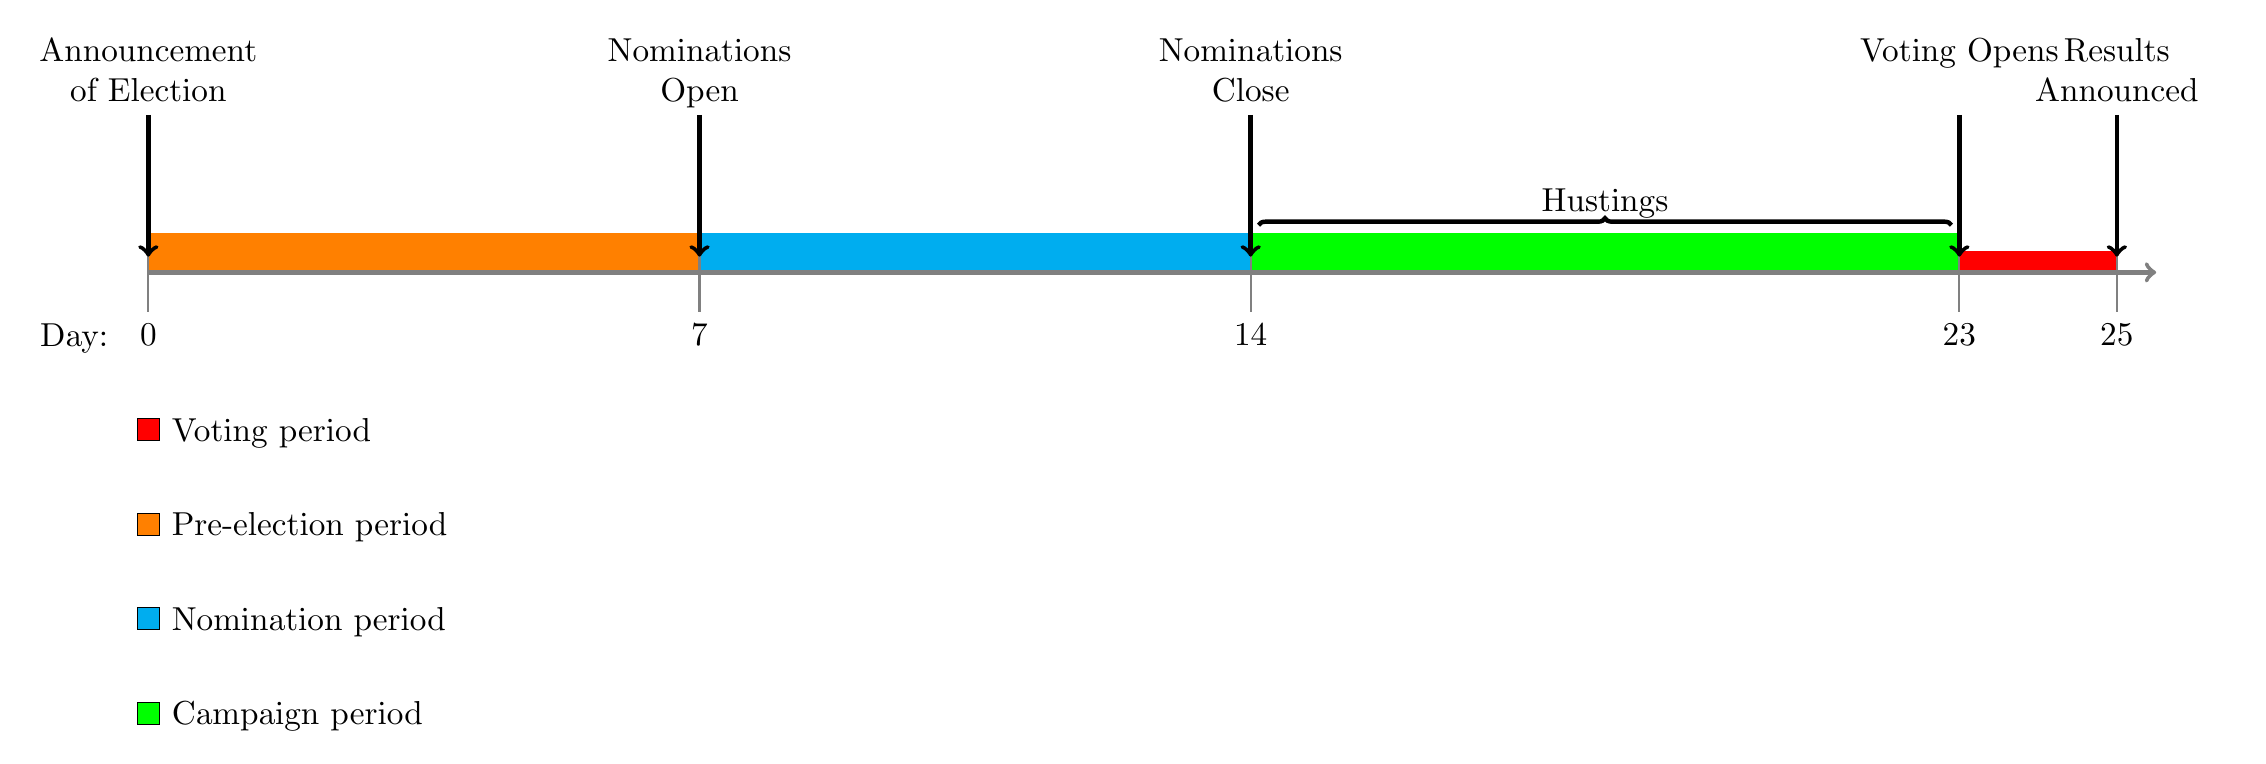
\begin{tikzpicture}[every node/.style={scale=1.2,text depth=0}]
        \node [label=right:Voting period,draw,fill=red] (key0) at (0,-2) {};
        \foreach \s/\e/\c/\n [count=\i,remember=\i as \j] in {0/7/orange/Pre-election,7/14/cyan/Nomination,14/23/green/Campaign} {
            \draw [\c,fill,line width=0] (\s,0) rectangle (\e,.5); % period highlighting
            \node [label=right:\n\ period,draw,fill=\c,below of=key\j] (key\i) {};
        }
        \draw [red,fill,line width=0] (23,0.27) rectangle (25, 0); % voting period
        \draw[ultra thick,black,decorate,decoration={brace}] (14.1,.6) -- (22.9,.6) node [black,midway,above] {Hustings};
        \draw[gray, ultra thick, ->] (0,0) -- (25.5,0); % axis
        \foreach \x/\e in {0/Announcement of Election,7/Nominations Open,14/Nominations Close,23/Voting Opens,25/Results Announced} {
            \draw[gray, thick] (\x,.5) -- (\x,-.5) node [black,below,at end] (day\x) {\x}; % ticks and day number
            \draw[black, ultra thick, ->] (\x,2.0) -- (\x,0.2) node [black,above=.5,at start,text centered,text width=66] {\e};
        }
        \node [left=.1 of day0] {Day:};
    \end{tikzpicture}
    \end{adjustbox}

    \section{Standing}
    \begin{itemize}
        \item All JCR members are entitled to stand in an election. However, you must be a finalist to be eligible for a sabbatical role.
        \item Before standing for a position, you should speak to the incumbent, JCR President, or JCR Chair.
        \item Candidates standing for JCR President, Senior Welfare Officer, Financial and Commercial Services Officer, and Senior Freshers’ Representative must meet with College Officers.
        \begin{itemize}
            \item They must contact the Senior Returning Officer to organise this before nominations open.
        \end{itemize}
    \end{itemize}

    \section{Nominations}
    \begin{itemize}
        \item To stand in an election, candidates must send their nomination to the Senior Returning Officer during the nomination period. The nomination must include:
        \begin{itemize}
            \item An A4 manifesto;
            \item Names of a Proposer and Seconder, who must be JCR members and not Executive Officers (past or present);
            \item For sabbatical roles, an A4 policy document.
        \end{itemize}
    \end{itemize}

    \section{Campaigning}
    \begin{itemize}
        \item During the campaign period, candidates standing in the election have the opportunity to campaign in-person and online.
        \item Only the candidate standing in the election, their proposer, and their seconder may campaign for the candidate (e.g. asking people to vote for the candidate).
        \item You must not unduly influence members to vote in a certain way or not to vote.
        \item No further campaign materials are permitted beyond candidates' manifestos and polcy documents (if applicable).
        \item If you have any questions on how campaigning works in JCR elections, you should reach out to the JCR Chair.
        \item All campaigning must follow the below guidance.
    \end{itemize}
    \subsection{In-person}
    \begin{itemize}
        \item In-person campaigning must take place during the campaign period and before the voting period.
        \item A candidate may campaign in-person for up to 4.5 hours, and their proposer/seconder may accompany them.
        \item A candidate must only campaign in-person in communal areas of College; i.e. areas that any member can access and not accommodation blocks.
        \item A candidate must tell the Senior Returning Officer the times, dates, and locations of their in-person campaigning.
        \item A candidate may advertise when they will be campaigning in-person through personal social media accounts.
        \item The Senior Returning Officer will organise the printing of manifestos to be displayed in College toilets.
        \item If in-person campaigning is not possible (due to serious adverse circumstances), the Election Officers may provide suitable alternatives.
    \end{itemize}
    \subsection{Online}
    \begin{itemize}
	\item A candidate, their proposer or seconder, may campaign online. This could include: publicising their manifesto; sharing the voting link; or messaging voters directly.
	\item Only personal online accounts may be used for campaigning.
    \end{itemize}

   \section{Executive Committee Hustings}
   \begin{itemize}
	\item All candidates will normally be invited to an Executive Committee Hustings, to hust in front of the Executive Committee at a time before the JCR Meeting Hustings, during the campaign period.
	\item	These will take the form of one candidate at a time being asked questions by members of the Executive Committee.
	\item Other candidates must not be present in the room.
	\item This may be done over live audio or video call.
	\item Candidates' attendance is strongly encouraged, however a failure to attend cannot be penalised.
    \end{itemize}

    \section{JCR Meeting Hustings}
    \begin{itemize}
        \item The election hustings will take place at a JCR meeting during the campaign period and
        before voting opens.
        \item All candidates standing for election must take part in the hustings.
        \item Candidates for President must prepare a 3-minute campaign video to played at the
        hustings.
        \begin{itemize}
            \item The video must be sent to the Head of Governance Committee 48 hours before the hustings.
        \end{itemize}
        \item Each prosper must give a one-minute speech followed by the candidate giving a two minute speech.
        \item For Presidential candidates, each candidate must sing a song, perform a poem or tell a joke. This may be done with their proposer and/or seconder. This will be followed by campaign videos.
        \item Each candidate may ask one question; followed by questions from incumbents, and then any other members.
        \item All candidates may respond to questions addressed at individual candidates.
        \item After questions, Presidential candidates may make a final concise statement.
    \end{itemize}

    \section{Voting and results}
    \begin{itemize}
        \item Voting is carried out during the voting period, which is between 24 and 168 hours, via the University's online voting system.
        \item A voting station may be set up and monitored by the Election Officers during the voting period.
        \item A member must not reveal how another member has voted.
        \item At the end of the voting period, the Election Officers will count the votes.
        \item The results will be announced on the stairs outside the bar. They should also be announced via an email to members and a post in the college Facebook group.
        \item Successful Presidential candidates traditionally perform a Kazu\footnote{A Kazu involves the candidate kicking a full can of Coca-Cola down the stairs in the foyer, throwing it over their head three times, and then opening it over their head.}.
    \end{itemize}
\end{document}